\subsection{Regra da dependência}

    \par A regra da dependência é o coração da Arquitetura Limpa, ela diz que o software deve ser organizado em camadas concêntricas, ou seja, com dependências apontando para dentro. Nesse sentido, para realizar a implementação dessa regra é necessário o uso de interface abstratas, que isolam as camadas internas (entidades e casos de uso) dos detalhes técnicos mais externos \cite{livro:martin:cleanarch}.

    \par Para realizar a implementação da regra da dependência, usa-se o Princípio da Inversão de Dependência (DIP), ao qual foi abordado anteriormente nesse trabalho. Ou seja, embora o fluxo de controle possa ir de uma camada interna para uma externa (por exemplo, um caso de uso que precisa atualizar a UI), a dependência do código-fonte é invertida \cite{livro:martin:cleanarch}.
    
    \par Para realizar a inversão  a camada interna define uma interface (uma porta) e a camada externa fornece a implementação concreta. Dessa forma, o código de alto nível que implementa as regras de negócio não depende do código de baixo nível que implementa os detalhes; pelo contrário, são os detalhes que devem depender das abstrações definidas pelas regras de negócio \cite{livro:martin:cleanarch}.
    
    \par Ao usar a Regra da Dependência Robert C. Martin explica que o software passa a ter uma arquitetura que implementa o mesmo padrão usado por sistemas que permitem o uso de \textit{plug-ins}. Os detalhes de baixo nível, como a UI, o BD, o servidor web e os \textit{frameworks}, são usados como \textit{plug-ins} para o núcleo do sistema, que contém as regras de negócio. Essa separação possibilita que as decisões sobre esses detalhes de implementação sejam adiadas e que eles possam até ser substituídos ou modificados caso seja necessário, com impacto muito baixo sobre as regras de negócio centrais do software, que por sua vez ficam estáveis e independentes \cite{livro:martin:cleanarch}.

    \par A Figura \ref{fig:figura_plugin_arch} demonstra a implementação desse conceito na prática, onde Robert C. Martin, mostra como os três componentes se comunicam aplicando a inversão de dependência. 

    \begin{figure}[H] % O [H] exige o uso do pacote float (veja abaixo)
        \centering
        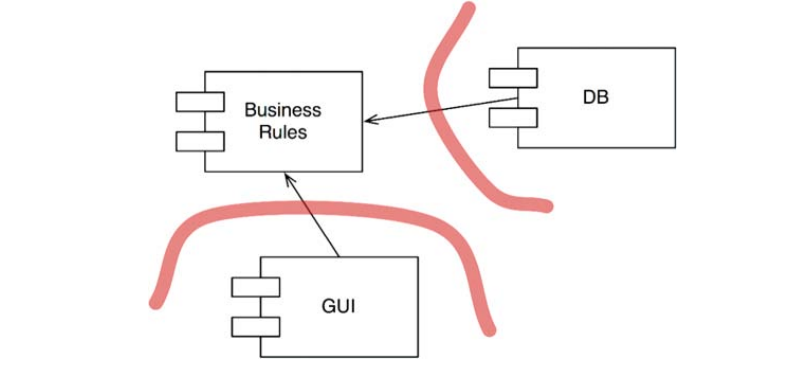
\includegraphics[width=1.0\textwidth]{figuras/clean_arch/plugin_arch.png}
        \caption{Colocando um \textit{plug-in} nas regras de negócio}
        \label{fig:figura_plugin_arch}
        \newcommand{\minhafonteum}{Fonte: \cite{livro:martin:cleanarch}}
        \minhafonteum
    \end{figure}

    As regras de negócio (Business Rules) não interagem diretamente com os detalhes de implementação, mas sim interfaces, que são como um \textit{plug-in}, que não fica acoplado ao núcleo do software, assim possibilitando a troca do BD ou da UI gráfica.
